% Page 022 — page imprimée 18
% Les Foires de Meyrueis


{\fontsize{10.2}{12.0}\selectfont

\begin{center}
{\Large\bfseries Les Foires de Meyrueis}
\end{center}

\vspace{0.75em}

Dès le Moyen Age, Meyrueis, située aux confins du Gévaudan et du Languedoc, apparaît comme une ville importante desservie par plusieurs chemins carrossables. Le bourg, également aux limites des Diocèses de Mende, Rodez et Nîmes, jouissait d’une renommée économique certaine.

Durant l’année foires et marchés se succédaient. C’était des espaces privilégiés de rencontre et d’échange, en particulier la foire de la St. Michel (29 Septembre) qui se tenait en continu jusqu’au 12 Octobre. Mais il y en avait sept autres !!!
C’est ainsi que l’on apprend, à l’article 39 des « consuetudines », (coutumes et usages de Meyrueis), octroyées en 1226, que tous les hommes « possédant une maison donnant sur l’une des trois rues « droites » sont tenus de nettoyer les rues ou passages depuis la Saint Michel jusqu’au 14\ieme jour suivant ».

Les gens de la campagne venaient vendre, chèvres et brebis, porcs, bœufs et mulets dont le commerce était florissant, ainsi que volailles et lapins. On venait y acheter les objets et ustensiles nécessaires à la cuisine, ainsi que le matériel agricole.
Ces foires attiraient beaucoup de monde. C’était une occasion de sortir et de rencontrer connaissances et amis. Des colporteurs proposaient des articles de mercerie, des toiles et des livres et brochures diverses. Il est probable que Pierre Belon, comme bien d’autres colporteurs, avait pu vendre, cachés sous rubans et dentelles, bibles ou psautiers, contribuant ainsi à l’essor de la Réforme.

\medskip

\textit{« Pour aller à la foire on s’endimanchait et, selon ses moyens et selon ce qu’on allait acheter ou vendre, on s’y rendait avec la jardinière, ou, le plus souvent, à pied. On faisait facilement vingt ou trente kilomètres en conduisant le bétail que l’on devait y vendre, et on partait vers minuit, une ou deux heures du matin suivant la distance... Si, comme c’était fréquemment le cas, on n’avait pu tout négocier à bon compte, on rentrait avec les bêtes invendues que l’on reconduirait à la prochaine foire... »}\footnote{Foires et marchés dans « Les Cévennes et la photographie ». Jean Noël Pelen et Daniel Travier p.205}

Dans le Thalamus de Meyrueis on découvre un article à la teneur singulière : « On appelle prostituées celles qui pèchent en public. Si cependant des femmes pèchent discrètement en évitant de s’exposer à la honte, qu’elles soient mariées ou non, il ne faut pas dire qu’elles sont des prostituées, et on ne doit pas, non plus les vouer à l’infamie ».

On peut penser à une prostitution tolérée au 13\ieme siècle, compte tenu de la durée de la Saint Michel qui était de 15 jours... Y-a-t-il eu changement avec l’installation de l’Eglise Réformée qui prêchait une certaine rigueur morale tout au long des 16\ieme et 17\ieme siècle ?

}

\begin{center}
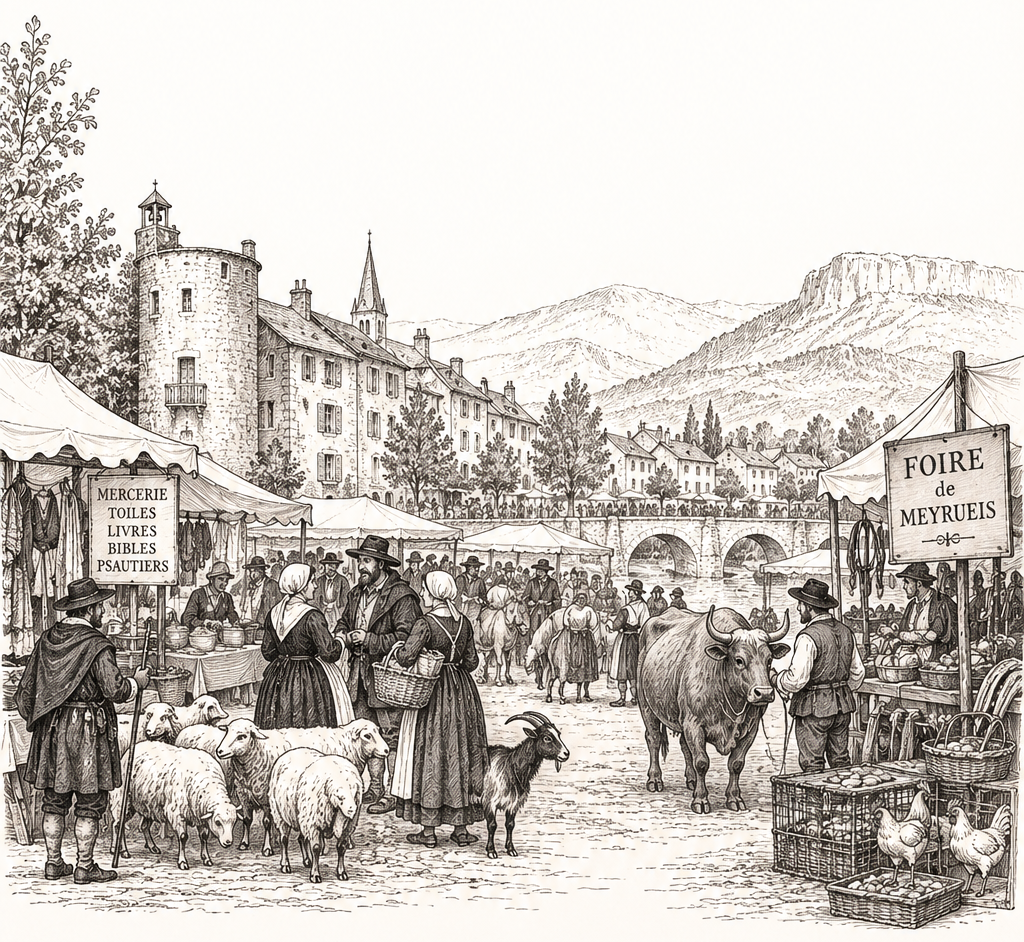
\includegraphics[width=0.7\textwidth]{imgs/022.png}
\end{center}


